\chapter{Background}
\epigraph{
In '87, Huey released this, Fore!, their most accomplished album. I think their undisputed masterpiece is "Hip To Be Square", a song so catchy most people probably don't listen to the lyrics - but they should! Because it's not just about the pleasures of conformity, and the importance of trends, it's also a personal statement about the band itself! Hey Paul!
}{Patrick Bateman before killing that massive stain Paul Allen with an axe}
Creating a cyborg is a massive cross disciplinary effort, and if a scope is not
clearly defined the background runs the risk of becoming equally massive.
The goal of the thesis is to create a hybrid neuro-digital system capable of
controlling a simple robot, and by extension to create a ``bridge'' between
neural and digital.
Each section in the background shares this bridge as a red thread, and
consequently topics that are not directly related to the thesis' goal are discarded.
The background is laid out as follows:
First \emph{Complex Systems} are introduced as a framework to discuss the computational
capabilities in a wide range of systems that exhibit system dynamics similar to
that of neurons.
Modeling neurons as a complex systems is a first step towards establishing a
common ``language'' between neural activity and digital logic.
%
Next, \emph{Material Computing} and \emph{Evolution In Materio}, EiM for short,
introduces computation done in unstructured matter through the process of
evolution. The goals of EiM are closely aligned to the goal of this thesis, as
both study massively parallel computation happening in physical matter shaped by
the process of evolution.
%
Next section, \emph{Neurons As Computers} introduces neurons with a strong focus
on their computational capabilities.
Building on the EiM section, this section motivates a necessary reduction of
scope, proposing a simplified model of the computing neuron and a medium of
communication between neuron and digital.
%
Finally, \emph{Reservoir Computing} is introduced, tying together the previous
sections by introducing the framework of reservoir computing in order to
establish a common ``language'' between neural cultures and digital.
\section{Complex Systems}
When designing systems in a top down manner it is imperative to control the
complexity of the system, or we are unable to reason about what it does and how
it does so.
By carefully managing complexity it is possible to make systems that are
\emph{complicated} in their makeup, yet with a simple, understandable behavior.
Larger systems can be assembled by combining smaller systems, and since each
subcomponent acts in a simple, predictable way, then so does the system as a
whole.
The effort necessary to understand the behavior of system as a whole is the same
as the sum of the effort required to understand each of its subsystems, and so
forth.
%
When studying most systems that occur naturally however, such as economical
systems, ecosystems, materials and how neurons together make up the mind, this
does not hold.
%
This is because the behavior we would like to model and predict cannot be traced
back to the individual agents of the system.
%
Although the individual parts of these \emph{Complex Systems} can be just as
complicated as in human engineered ones, it is the \emph{Non-linear} dependence
between these parts that decides the behavior of the system as a whole.
%
It is these complex interactions that allows systems to spontaneously \emph{Self
  Organization} and adapt to change.
%
\subsubsection{Attractors}
% beskrivelse
The ``force'' that drives the self organization of complex systems is feedback.
Positive feedback loops can cause a chain reaction that completely alter the
dynamics of a system, while negative feedback acts as a dampener, allowing the
system to have some measure of stability.
Systems with mostly negative feedback are ordered and predictable, while systems
with mostly positive feedback are chaotic and unpredictable, seemingly random.
This interplay between dampening and positive feedback gives rise to an
%
\emph{attractor landscape}, where the \emph{state space} of a system gets
partitioned into one or more attractors.
%
Figure ?? shows a simple map of a state space for a system with four
\emph{attractors} and the current state of a system represented by a point.
This space is not a physical one, each point on the line describes the systems
behavior as a whole and adding a velocity to a system moving along the state
space violates this constraint.
In simple terms, the state can only move towards lower energy.
%
The behavior of a system 
%
% Similarily, although the y axis is labeled energy this is not necessary energy
% in a physical sense, for many systems a more fitting description is stability of
% behavior.
% In order to move the behavior of the system energy must be introduced to the
% system from the outside, and if enough energy is introduced the system may fall
% into a different attractor.
% In fig ?? the systems behavior is currently in an attractor labeled B, and
% energy can be applied either towards A or C, but it takes much more energy to
% move the system towards C.

%
\subsubsection{Next up}
\subsubsection{Noe om observation scale?}
It is at \emph{The edge of chaos} where positive and negative feedback are
evenly matched that systems can spontaneously self organize without being chaotic.
%
In the context of evolution seems necessary for systems to exist at this edge of
chaos.
For a plant it is essential to be able to respond to changes in light
conditions, but it is equally important to maintain integrity.
No two pines are alike, but they all have bark on the outside and they all grow
upwards.
In a swiss watch everything stops working if a single spring or cog is replaced
with a slightly different one, yet in nature no two animals or plants are alike.
The \emph{robustness} of complex systems goes beyond mere survival, it's what
makes the incremental changes of evolution possible in the first place!
%
While the neurons that make up neural networks are both complex and complicated,
it is in the interactions between them that computation happens, and this
complex interaction can be modeled in a much simpler system.
\par
\begin{figure}[h!]
  \centering
  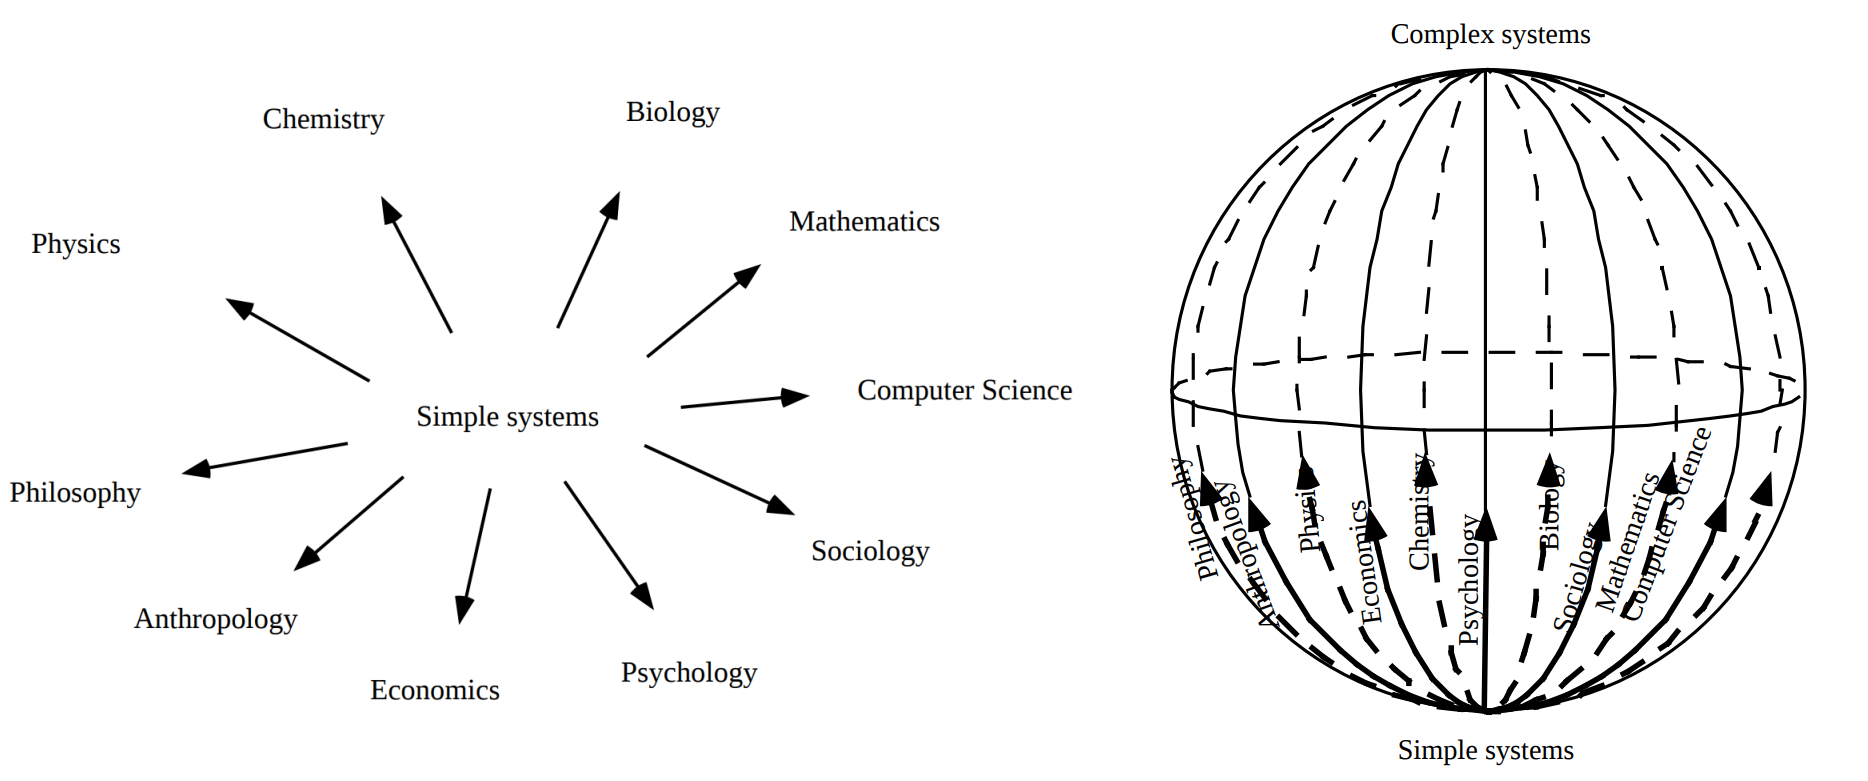
\includegraphics[width=0.6\textwidth]{fig/BarYamCX.png}
  \caption{From Bar Yam book.}
  \label{figCX}
\end{figure}
\subsubsection{Cellular Automata}
A \emph{Cellular Automaton}\footnote{Singular: Automaton, Plural: Automata}, CA
in short, is a simple discrete model of a single cell which changes between a
discrete set of states based only on its immediate neighbors.
Figure \ref{figCA22} shows an example of a \emph{rule set}, or \emph{transition
  table} for a cellular automaton with only two states, and an initial
configuration, or ``seed'', which over several steps forms a pattern.
%
One of the pioneers in the field of CAs, Stephen Wolfram suggested that under
certain conditions CAs were capable of computation [cite Wolfram: Universality
and complexity in cellular automata].
%
Cellular automatas have been shown capable of solving global problems such as
contour-extraction \cite{sipper_emergence_1999} where the problem is expressed
as the seed and a global solution emerges from the local interaction of cells.
Wolframs hypothesis of universal computation has also been proven correct, in
fact even a simple 1D cellular automata such as in \ref{figCA22} has been proven
sufficient to simulate a turing machine [Cite Matthew Cook],
but as Sipper puts it: ``This is perhaps the quintessential example of a slow
bullet train: embedding a sequential universal Turing machine within the
highly parallel cellular-automaton model.''\par
% 
% Her var jeg. Skriv noe om at vi tar det for gitt at utregning kan skje, vi
% bryr oss ikke om hvordan, men hva slags conditions kreves per Langton.
%
In figure [figur av class 1 - IV CA] four cellular automatas are shown,
each classified per Wolframs CA classification.
The fourth class which ``yields complex patterns of localized
structures'' shows complex behavior which Wolfram suggested was the sort of
behavior necessary for computation to occur spontaneously.
%
As a model for neurons it is sufficient to know that they are capable of
computation and under which circumstances rather than knowing exactly what they
are computing.
%
In Langton's pioneering paper \emph{Computation on the Edge of Chaos}
\cite{langton_computation_1990} the space of possible transition tables for one
dimensional cellular automata with two states, such as \ref{figCA22} is explored.
What Langton discovered was that the ratio between states leading to life and
death (black and white cells respectively) was analogous to how temperature
causes phase changes in materials.
This is not suprising, as one would expect rulesets where most transitions lead
to death will lead to a stationary system analogous to ice, while a transition
table favoring life and death equally leads to a chaotic system analogous to a
gas.
What was suprising however, was that at the edge between periodic and chaotic
there existed a \emph{Critical Phase}, shown in \ref{figCAegg}.
This effect also happens in materials in what is called a 2nd order phase
change, in which the material is neither gas, liquid or solid, but exhibits all
three in local substructures that can be found on all scales, from macroscopic
to microscopic.
The takeaway from the model of cellular computation is the idea that there are
certain criterias that enable computation to occur spontaneously, and that
neurons actively attempt to reach this critical phase.
\begin{figure}[h!]
  \centering
  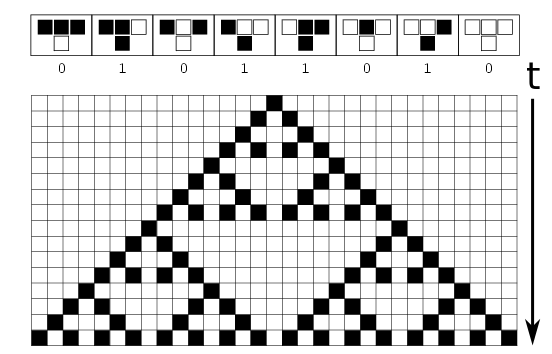
\includegraphics[width=1\textwidth]{fig/ca22.png}
  \caption{Should add a time axis to drive the point home that these are 1D}
  \label{figCA22}
\end{figure}
\begin{figure}[h!]
  \centering
  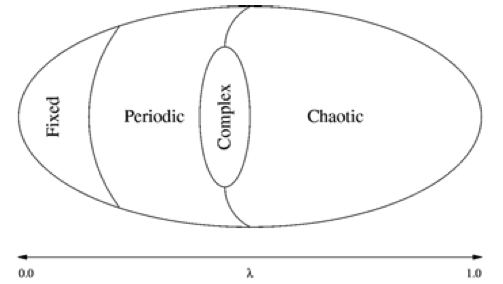
\includegraphics[width=1\textwidth]{fig/Langtons_egg2.png}
  \caption{Langtons egg}
  \label{figCAegg}
\end{figure}
\section{Material Computing}
Modeling neurons as cellular automata gives an idea of how neurons organize
themselves into computationally capable networks and how this computation may
look like, but the question of how to make sense of these dynamics and utilize
them.
Before tackling neurons it is necessary to extend our model to the physical
realm and develop a model that can be extended to perform computation.
A very natural extension of the CA model is \emph{material computing} in which
the atoms that make up matter locally interact in similar ways to CAs.
%
Two pioneers in this field were the british duo Pask and Beer which studied how
unstructured matter could be used to perform computational tasks.
%
In one experiment [cite ???] the duo used silver in an acidic solution which
would form short-lived silver filaments when subjected to electric currents.
%
By tuning the various knobs controlling parameters such as voltage this solution
could be made to perform the task of tone discrimination, proving that
unstructured matter could in fact perform computation.
%
In Langtons CAs the goal was not to compute, but to explore what conditions were
necessary for computation to occur, while Gordon and Pask sought to actually
compute by observing how the matter reacted to sound and tuning the parameters
in response.
%
Tommaso Toffoli argues that ``Nothing makes sense in computing except in the
light of evolution'' in his eponymous paper [cite TT], which separates Langtons
compute capable CAs and the tone discrimination which had been evolved by
repeatedly observing its performance and altering the parameters accordingly.
%
% Hmm hmm hmm
A corollary of the turing completeness of cellular automatas is that CAs can be
``tuned'' in a rather heavy handed way to compute, but a more interesting
conjecture is that a CA with a random seed will eventually exhibit local
self-replicating behavior, spontaneously giving rise to what Toffoli would
regard as computation, or possibly even as life.\par
%
Whereas the pioneers in material computing sought to perform specific tasks with
their experiments more recent work has been made for general computation.
One approach is \emph{Evolution In Materio} where various materials have their
parameters tuned algorithmically to perform a transformation between input and
output.
A recent effort is the NASCENCE project which has developed a physical device,
``mecobo'' that can host a variety of materials which can then be interacted
with using an array of electrodes.
By using the same basic loop as the early material computing reasearchers the
Mecobo board has been used to create XOR logic gates using unstructured carbon
nano-tubes [Cite Odd paper 1].
%
% This gives latex error about missing dollarsign, but upon inserting text is no longer
% bold...
\subsubsection{(DS)^2}
%
In the introduction Fernando's water bucket computer was briefly mentioned [cite
bucket].
In their paper they refer to the bucket as a ``liquid brain''\footnote{Also in
  quotation marks in the original paper}, performing calculations by observing
the resulting wave pattern made by small motors.
Unlike its biological counterpart the ``liquid brain'' does not evolve over
time, in fact it has no structure to evolve at all, at least not at the chosen
scale of observation.
%
$(DS)^2$ is shorthand for dynamic systems with \emph{dynamical structure}, and
materials that exhibit this behavior can be used to study and model biological
systems.
In these material systems the \emph{state space}, that is the set of reachable
states, and the transition function between them evolve over time in tandem with
the systems dynamics, both shaping them and being shaped by them.
%
In [cite Odd Rune EiM (DS)2] Odd Rune shows that a mixture of table salt and
water exhibits (DS)2 behavior using the mecobo board by showing that the systems
response to perturbation evolves over time.
%
Simalirily, experiments using simulated artificial spin ice [Cite Johannes]
shows that in a lattice of nano-magnets several underlying microstates map to the
same macro-state as shown in fig ??
This highlights the importance of observation level when describing systems.
One could choose to... Something something.

\section{Computing Neural Networks}
Material computing provides both a theoretical framework and practical
approach for modeling and interacting with the computational capabilities of
living neural networks.
%
The $(DS)^2$ viewpoint is a very natural fit when modeling how neurons organize
into networks.
The structure in a neural network continously evolves as each neuron
individually seeks out other neurons to forge new connections while letting old
connections wither and die off.
The dynamics of a neural network is the electro-chemical communication between
neurons in the network.
These signals are obviously shaped by the topology of the neural network, but
they are also the driving force between the continued evolution of the networks
topology in ways that we only have a rudimentary understanding of.
%
Although both table salt and neural networks exhibit $(DS)^2$ behavior only the
neurons do this on purpose.
When viewing Pask's tone discrimination experient from a $(DS)^2$ viewpoint we
can catch a glimpse of the same process that shaped the rules governing neural
self organization.
Although this was not the view of the experimenter, the tuning of parameters
performed by Pask altered how silver filaments formed and decayed, which can be
viewed as a rudimentary approximation of how neurons form connections.
%
In Pask's experiment the observer tuning the knobs served the same role as
evolution did in shaping neurons, and neither force were particularily concerned
about exactly what the underlying structure of the material did as long as the
behavior of the material performed as desired on a macro-scale.
%
\subsubsection{The Computing Neuron}
The neuron, or nerve cell, is the basic building block of both the human brain
and the nerve system.
The culmination of billions of years of evolution, the neuron is a vastly
complex entity, featuring complex chemical pathways and gene regulatory
networks.
However, as discussed in the section on complexity, this behavior is nescessary
in order for evolution to function.
As a corollary, most of the complexity of the neuron is not nescessary for it to
function, it is simply a byproduct of evolution, an implementation detail.
It is the view of the author that the behavior of a neural network can be
modeled with a much simpler neuron such as in artificial spiking neural
networks.\par
Although the computation performed by neurons can be modeled with simpler
models, the fact of the matter is that the cyborg project utilizes real neurons
rather than a digital approximation, so a cursory introduction of the neuron is
in order.
While there exists a multitude of different neurons in the human body it is
sufficient to consider a simplified model neuron, shown in fig [a figure of a
neuron].
The three three main parts are the body, or \emph{Soma}, the \emph{Dendritic
  network} and the \emph{Axon}. 
The dendritic network acts as a receptor sensing electrical activity around the
neuron, while the axon transmits electric pulses to neighboring cells.
The connection between two neurons is called a \emph{Synapse}.
%
In addition to chemical signals neural networks communicate and regulate their
behavior through chemical signals.
These chemical signals, known as neurotransmitters, correlate strongly with
electrical activity however, thus measuring the chemical gradients in neural
networks is not a priority from a compuational perspective.
\subsubsection{Neural Dynamics}
The ``medium'' of communication between neurons chosen as the observable macro
state, that is the dynamics we are interested in measuring for the neural
network are electrical bursts of activity, known as spikes.
Figure [fig of waveform] shows recorded activity from an electrode.
Each electrode measures the activity of the surrounding neurons rather than the
state of a single neuron.
Given that spikes propogate through the network in a cascading manner this
level of observation is sufficient and more fine grained measurements is not a
priority.
Over time these dynamics evolve in tact with the structure of the network, as
expected in the section on $(DS)^2$.
Not only does the dynamics of the neural network change like the table salt
experiment, it moves in the complexity space as shown in [fig neuro complexity
graph] towards a critical phase as discussed in the section on cellular automata.
%
\subsubsection{Artificial Neural Networks}
In recent years ANNs\footnote{Or rather, the advent of hardware capable of
  efficiently running and training them.} (shorthand for artificial neural
network) have revolutionized AI due to their ability to solve hard
classification problems such as image recognition.
The simplest, and most successful variation is the \emph{feed forward} topology
shown in \ref{figFFANN} in which each layer only interacts with the layer
directly in front and behind it.
Shown in \ref{figNeuronModel}, the model for a single neuron consists of a
summing function that calculates a weighted sum of incoming connections and a
function that calculates the outbound activation of that neuron.
More advanced models of neurons often retain state from their previous
activation, one such variant being the spiking neuron which emulates the
biological neuron more faithfully.
Networks with neurons that retain state can have more interesting topologies
where the connections between neurons can go in all directions.
Cleary recurrent spiking neural networks should be more capable than feed
forward networks, if nothing else for their ability to encode time-series as
part of their state, yet the simple, non-spiking variant has proven much more
successful.
This gap stems from the relative simplicity of the fitness landscape of simpler
network topologies which allows training algorithms to manually adjust the
weights between layers iteratively until a good result is achieved.
In back-coupled networks however the relation between cause and effect is far
more obscure, thus algorithms which essentially assign blame and alter weights
based on this are unable to cope with these topologies.
\begin{figure}[h!]
  \centering
  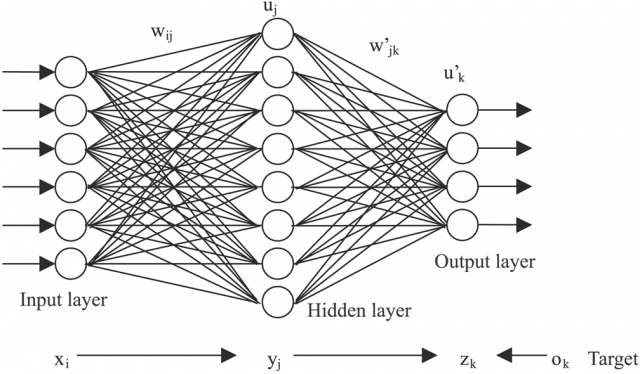
\includegraphics[width=0.7\textwidth]{fig/FFANN.png}
  \caption{A feed forward ANN.}
  \label{figFFANN}
\end{figure}
\begin{figure}[h!]
  \centering
  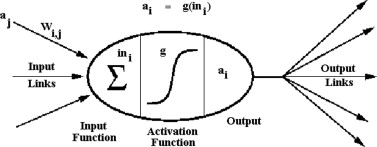
\includegraphics[width=0.7\textwidth]{fig/ArtificialNeuron.jpg}
  \caption{A feed forward ANN.}
  \label{figNeuronModel}
\end{figure}

% Få inn RC fig tidligere
\section{Reservoir Computing}
Material computing has provided a tractable model of how the neuron computes and
how to physically interface with them.
However, still absent is a model that allows us to actually access the
computational capabilities.
In fact, from the field of material computing Susan Stepney extends the
following warning ``the biological substrate is extremely complex and
complicated, having evolved over billions of years to exploit specific
properties. In some sense, biological substrate is as far (or further!) removed
from a primitive substrate as are our own designed abstract digital
computational media.''
%
As the heading indicates, the ace up our sleeve comes in form of \emph{Reservoir
  Computing}, a technique that fittingly enough originated from the study of
ANNs of the back-coupled variety[Cite Jaeger][Cite Maass].
In [Cite Jaeger] randomly connected neural networks are used to solve
classification problems, forgoing training the network altogether.
Instead the randomly generated network was used as a \emph{reservoir} of
dynamics that reacted to the input while a simple linear output function had to
be trained.
The principle behind reservoir computing is to employ a complex system as a
reservoir which, as Schrauwen puts it \cite{schrauwen_overview_2007} ``... acts
as a complex nonlinear dynamic filter that transforms the input signals using a
high-dimensional temporal map, not unlike the operation of an explicit, temporal
kernel function.''
Figure \ref{figRC} shows this setup, in which input perturbs a reservoir and the
resulting dynamics is classified using a linear filter.
%
In order to explain why this works, schrauwen makes a comparison to the the
machine learning technique of source vector machines work, as shown in fig
\ref{figSVM}. The general idea behind an SVM is to expand the input into a
higher dimensional ``feature space'', which in the figure is represented by the
transition from 2D to 3D.
% Altså sensitivitet til input conditions
Systems with complex behavior can behave remarkably different depending on
certain subtle nuances in the input while exhibiting a large tolerance to
variations for other inputs.
To see why, consider how the behavior of a complex system can be described by
which attractor it is currently in as a result of some initial condition.
%
In his comparison Schrauwen points out the major difference between SVMs and
reservoir computing which is that reservoirs can implicitly encode temporality
of input by changing their state.

% Schrauwen points out two major differences between SVMs and RCs.
% First, SVMs only implicitly expands the input to high dimensional space in order
% to make the problem tractable, while reservoirs do not.
% Secondly, kernels are not capable of handling temporal signals.
% %
% The second difference is very important, it is what allows reservoirs to
% implicitly encode temporal signals in their dynamics, making reservoirs a
% natural fit for tasks such as speech recognition.
% % cite Biologically Plausible Speech Recognition with LSTM Neural Nets Alex
% % Graves, Douglas Eck, Nicole Beringer, Juergen Schmidhuber
% % 
% In other terms, the properties that make complex systems so hard to work with
% such as sensitivity to initial conditions also allow them to discern very subtle
% nuances in input, and their complex behavioral patterns causes the systems to
% change their behavior to new input based on previous input.
% %
% In light of this, asking how to build a computer using Langton's automatons is
% the wrong question, instead the focus should be on how exploit the computation
% that is already occuring.\\
% There are many examples of reservoirs which have been successfully exploited:
% In \cite{jaeger_adaptive_2003} an \textit{echo state network} 
% is utilized to solve classification problems.
% More esoteric reservoirs have been used, for instance in
% \cite{natschlager_liquid_2002} the idea of reservoir computing is taken quite
% literally using a bucket of water as a reservoir.\\

\begin{figure}[h!]
  \centering
  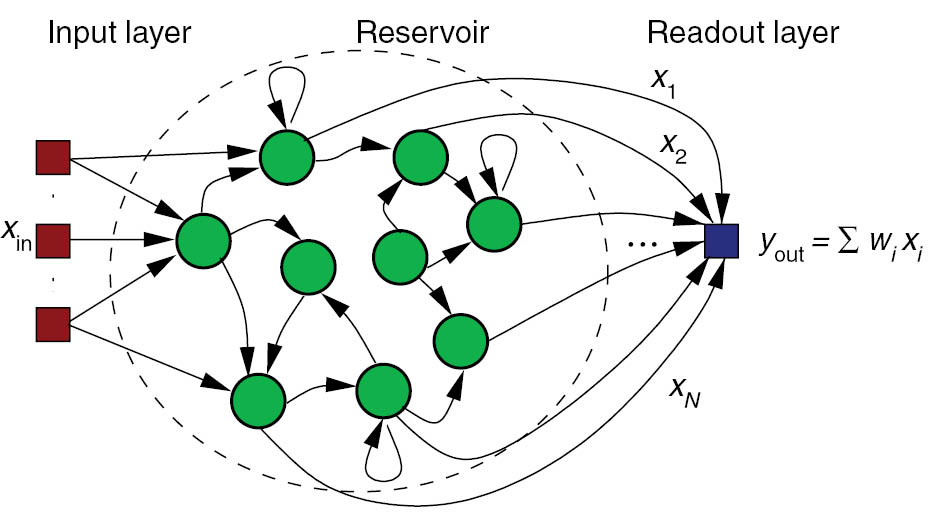
\includegraphics[width=0.7\textwidth]{fig/RC.jpg}
  \caption{A feed forward ANN.}
  \label{figRC}
\end{figure}
\begin{figure}[h!]
  \centering
  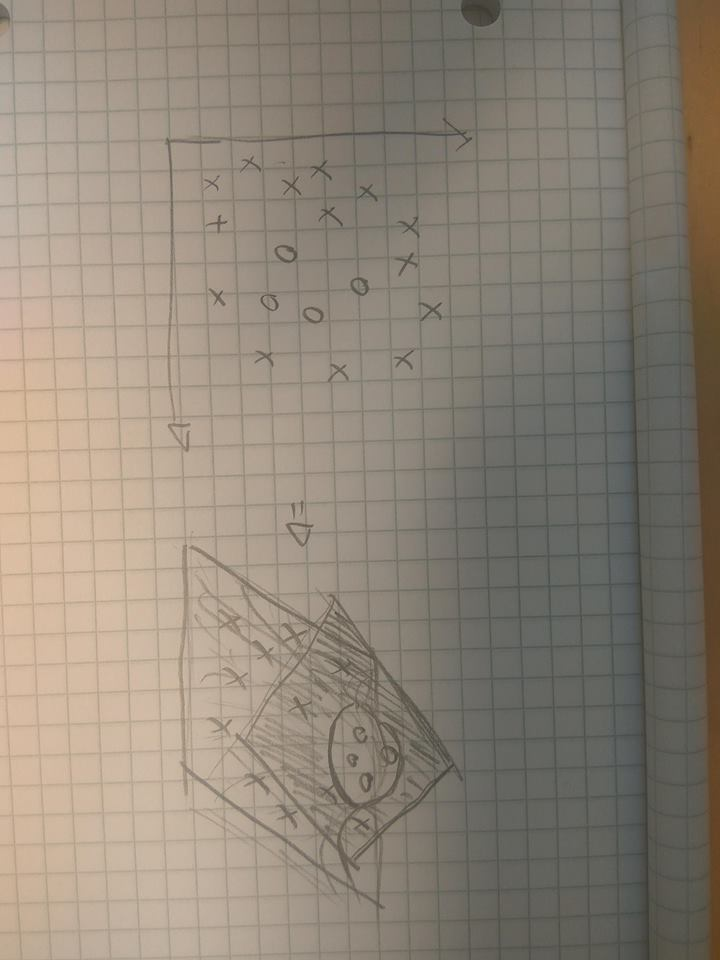
\includegraphics[width=0.6\textwidth, angle =90]{fig/transform.jpg}
  \caption{Should say ``kernel function'' or similar on top of the arrow}
  \label{figSVM}
\end{figure}
\subsection{Linear and nonlinear output layers}
TODO: Elaborate on the use of linear vs nonlin classifiers.

\cleardoublepage

%%% Local Variables:
%%% mode: latex
%%% TeX-master: "../main"
%%% End: